\documentclass[12pt]{article}
\usepackage[utf8]{inputenc}
\usepackage[english]{babel}
\usepackage{graphicx}
\usepackage{float}
\usepackage{caption}
\usepackage{subcaption}

\setlength{\oddsidemargin}{0in}
\setlength{\evensidemargin}{0in}
\setlength{\textwidth}{6.5in}
\setlength{\topmargin}{-.3in}
\setlength{\textheight}{9in}
\setlength{\parskip}{1em}

% \pagestyle{empty}
\graphicspath{ {images/} }
% ___________________________________________________________________

\begin{document}

\begingroup  
  \centering
  \large Report: Experiments on $\alpha$ updates \par
  \large Arijus Pleska \par
\endgroup
% ___________________________________________________________________

\par This report assesses experiments on reproducing $\alpha$ parameters used in the synthetic data generation process. Note that the report is structured in the following order: at the start, the rationale of the used Bayesian methods are covered; then, the experiment settings are defined; in the following stage, we assess the experiment results; finally, the identified issues are outlined to be discussed during the following meeting.
% ___________________________________________________________________

\section*{Preliminaries}

\par In order to understand the experiment experiment settings, it is necessary to be familiar with the auto-regressive and non auto-regressive $\alpha$ priors as well as the Metropolis--Hastings (M--H) algorithm.

\par The previously introduced priors can be expressed as follows:

% ___________________________________________________________________

\section*{The Experiment Settings}

\par The intention of the carried experiments is to identify the optimal settings for the Metropolis--Hastings algorithm application. 
To start with, I have generated a synthetic corpus; the parameters used in the corpus generation will allow to assess the performance achieved in the experiments. The corpus generation parameters are set as follows:
\begin{itemize}
  \item The number of topics: K = 2;
  \item The number of documents (time-slices): T = 20;
  \item The size of vocabulary: V = 10;
  \item The number of words per document t: $N_t \sim \mbox{Pois}(\lambda),\quad \lambda = 1000$.
\end{itemize}
Further, to consider the initial settings of $\alpha_k$ development over documents, $\alpha_0$ is a sine curve and $\alpha_1$ is a cosine curve; the corresponding softmax expressions of the curves, i.e $\mu = \mbox{softmax}(\alpha)$, are illustrated in Figure 1 below.
\begin{figure}[H]
  \centering
  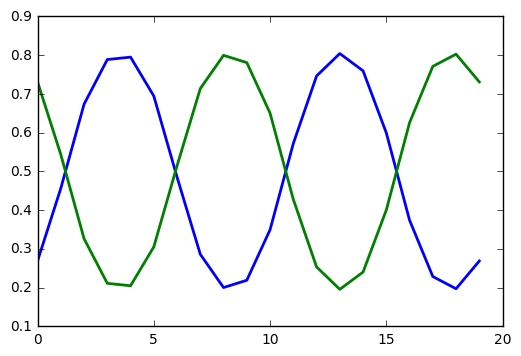
\includegraphics[width=0.5\textwidth]{alpha_initial}
  \caption{The values of $\mbox{softmax}(\alpha)$ used in the generative process.}
  \label{fig:mu}
\end{figure}
Speaking of $\beta$, it was initially predefined and kept constant throughout the dynamic generative process; $\beta$ is illustrated in Figure 2 below.
\begin{figure}[H]
  \centering
  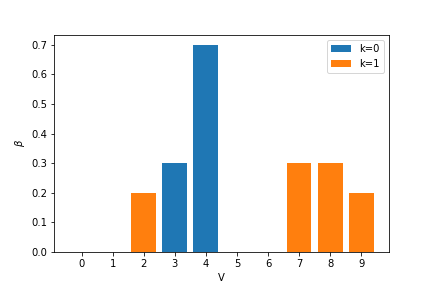
\includegraphics[width=0.5\textwidth]{beta_initial}
  \caption{The values of $\beta$ used in the generative process.}
  \label{fig:beta}
\end{figure}
Note that the latter $\beta$ values were applied to the autoregressive topic model for the $\alpha$ update experiments.
% ___________________________________________________________________

\section*{The experiment results}

\par The first experiment is focused on discovering the choice of the variances. To be more specific, the alpha update is based on three different variances were used: the `initial' variance $\sigma^2_0I$ to induce $\alpha_t$ at $t=0$, the `basic' variance $\sigma^2I$ to induce $\alpha_t$ at $t>0$, and the `proposed' variance $\delta^2I$ to induce $\alpha'_t$ at $t=0$; also, note that $\alpha'_t$ at $t>0$ were induced using the `basic' variance.

\par For both experiments, the number of autoregressive iterations was set to $500$ and $\sigma^2$ was set to $0.01$. The resulting plots of $\mu$ with different values of $\sigma^2_0$ and $\delta^2$ are illustrated in Figures 3, 4, 5 below.

\begin{figure}[H]
        \begin{subfigure}[b]{0.33\textwidth}
                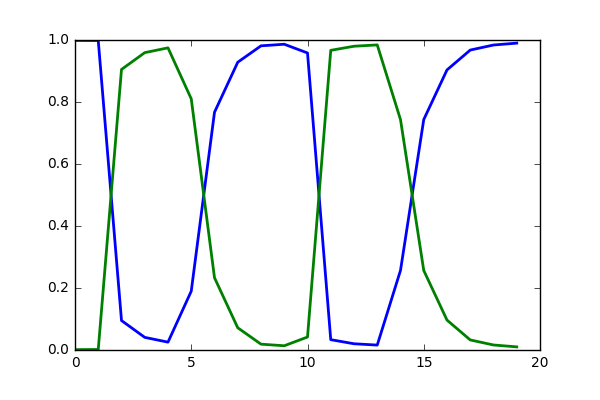
\includegraphics[width=\linewidth]{init-1_prop-05}
                \caption{$\sigma^2_0=1,\quad \delta^2=0.5$}
                \label{fig:gull}
        \end{subfigure}%
        \begin{subfigure}[b]{0.33\textwidth}
                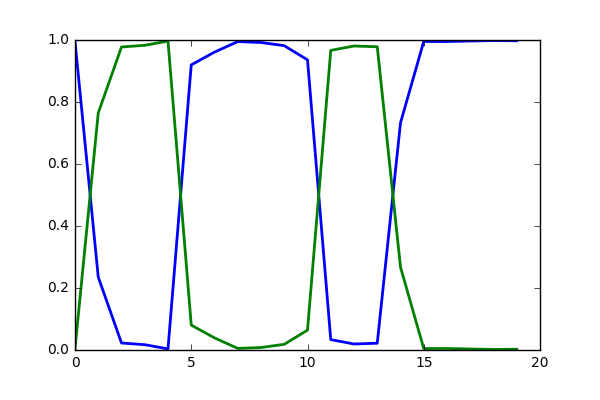
\includegraphics[width=\linewidth]{init-1_prop-2}
                \caption{$\sigma^2_0=1,\quad \delta^2=2$}
                \label{fig:gull2}
        \end{subfigure}%
        \begin{subfigure}[b]{0.33\textwidth}
                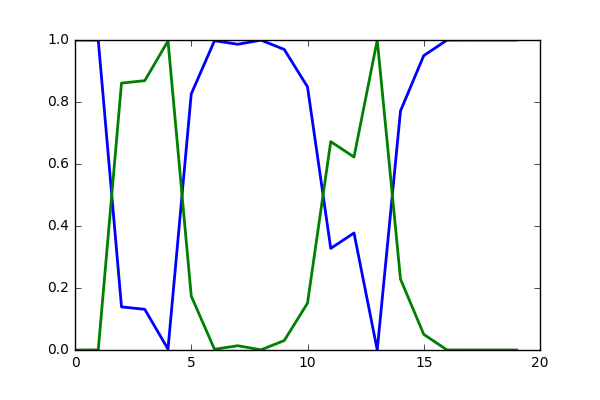
\includegraphics[width=\linewidth]{init-1_prop-5}
                \caption{$\sigma^2_0=1,\quad \delta^2=5$}
                \label{fig:tiger}
        \end{subfigure}
        \caption{$\mbox{softmax}(\alpha)$ with the lowest value of the initial variance.}\label{fig:animals}
\end{figure}
\begin{figure}[H]
        \begin{subfigure}[b]{0.33\textwidth}
                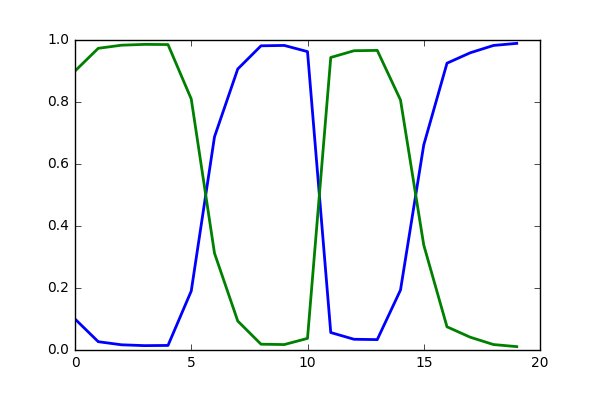
\includegraphics[width=\linewidth]{init-5_prop-05}
                \caption{$\sigma^2_0=5,\quad \delta^2=0.5$}
                \label{fig:gull}
        \end{subfigure}%
        \begin{subfigure}[b]{0.33\textwidth}
                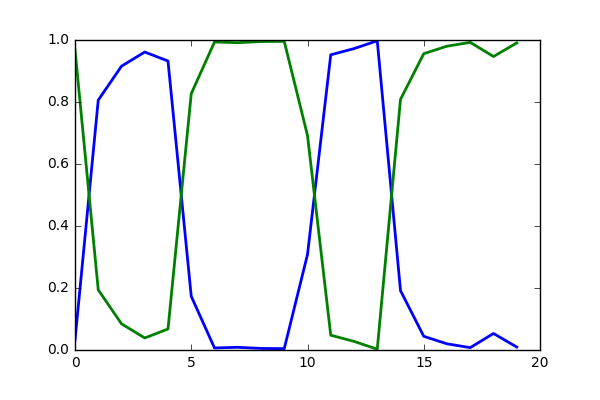
\includegraphics[width=\linewidth]{init-5_prop-2}
                \caption{$\sigma^2_0=5,\quad \delta^2=2$}
                \label{fig:gull2}
        \end{subfigure}%
        \begin{subfigure}[b]{0.33\textwidth}
                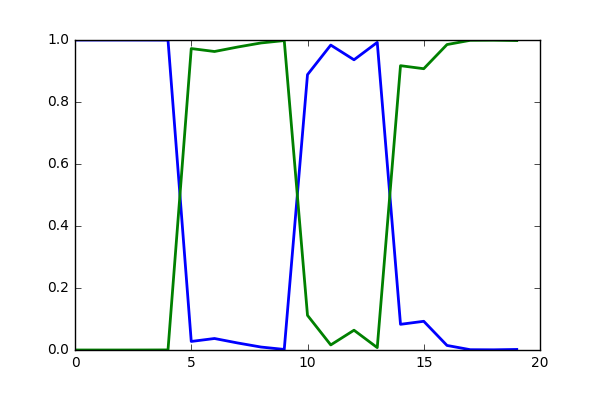
\includegraphics[width=\linewidth]{init-5_prop-5}
                \caption{$\sigma^2_0=5,\quad \delta^2=5$}
                \label{fig:tiger}
        \end{subfigure}
        \caption{$\mbox{softmax}(\alpha)$ with the average value of the initial variance.}\label{fig:animals}
\end{figure}
\begin{figure}[H]
        \begin{subfigure}[b]{0.33\textwidth}
                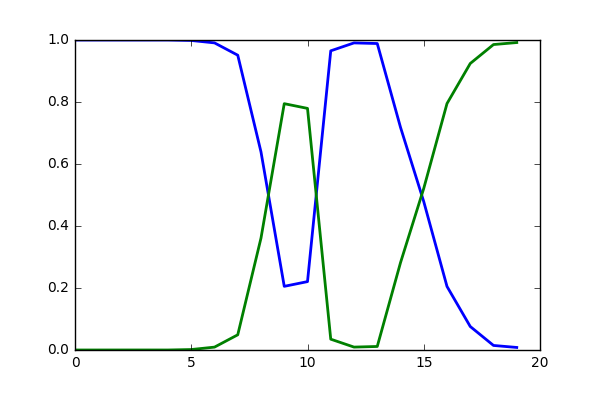
\includegraphics[width=\linewidth]{init-10_prop-05}
                \caption{$\sigma^2_0=10,\quad \delta^2=0.5$}
                \label{fig:gull}
        \end{subfigure}%
        \begin{subfigure}[b]{0.33\textwidth}
                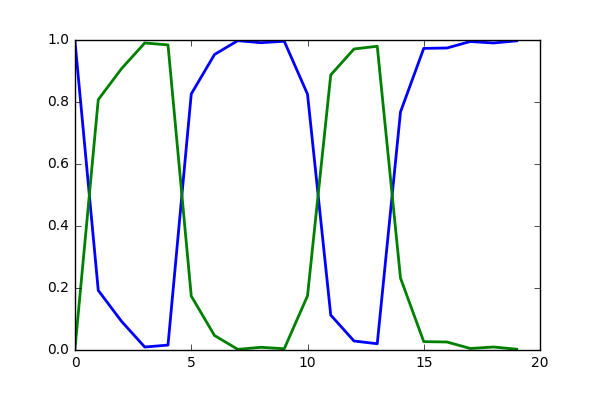
\includegraphics[width=\linewidth]{init-10_prop-2}
                \caption{$\sigma^2_0=10,\quad \delta^2=2$}
                \label{fig:gull2}
        \end{subfigure}%
        \begin{subfigure}[b]{0.33\textwidth}
                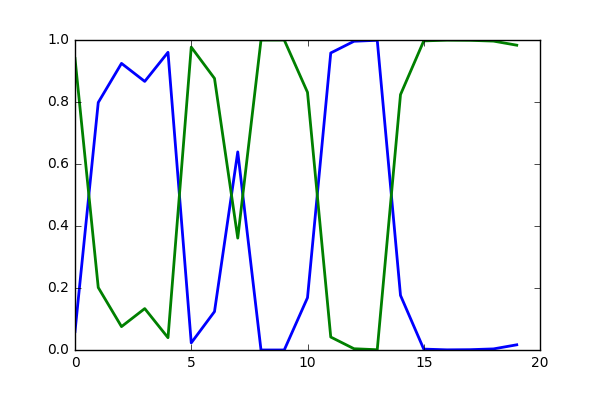
\includegraphics[width=\linewidth]{init-10_prop-5}
                \caption{$\sigma^2_0=10,\quad \delta^2=5$}
                \label{fig:tiger}
        \end{subfigure}
        \caption{$\mbox{softmax}(\alpha)$ with the highest value of the initial variance.}\label{fig:animals}
\end{figure}


\par The second experiment was carried to determine the impact of the $\alpha$ update in recovering the original topic fluctuations in the synthetic corpus. For this reason, the autoregressive part of the dynamic topic was disabled. The topic assignments to the documents of the last iteration are visualised in Figure 6 below.

\begin{figure}[H]
  \centering
  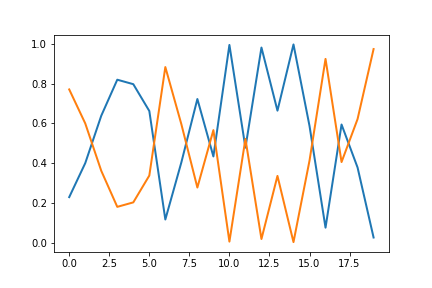
\includegraphics[width=0.5\textwidth]{thetas}
  \caption{The topic assignments to the documents.}
  \label{fig:mu}
\end{figure}
% ___________________________________________________________________

% \section*{Observations}

% \par For the last section of this report, I have set some questions to be addressed during next meeting; these are listed below:
% \begin{itemize}
%   \item In some cases, the larger number of iterations reduced the performance in reproducing the initial $\alpha$;
% \end{itemize}
% ___________________________________________________________________


%\bibliography{report_mh_alpha-update}{}
%\bibliographystyle{plain}
\end{document}
